\documentclass[12pt,letterpaper,noanswers]{exam}
%\usepackage{color}
\usepackage[usenames,dvipsnames,svgnames,table]{xcolor}
\usepackage{natbib}
\usepackage[margin=0.9in]{geometry}
\renewcommand{\familydefault}{\sfdefault}
\usepackage{multicol}
\newcommand{\vc}[1]{\boldsymbol{#1}}
\pagestyle{head}
\definecolor{c02}{HTML}{FFBBBB}
\definecolor{c03}{HTML}{FFDDDD}
\header{AM 111 Problem Set 05}{}{{\colorbox{c02}{\makebox[2.8cm][l]{Due Fri Oct 6}}}\\at 5pm}
\runningheadrule
\headrule
\usepackage{diagbox}
\usepackage{graphicx} % more modern

\usepackage{amsmath} 
\usepackage{amssymb} 

\usepackage{hyperref}

\usepackage{tcolorbox}
\usepackage[framed,numbered,autolinebreaks,useliterate]{mcode}


\def\been{\begin{enumerate}}
\def\enen{\end{enumerate}}
\def\beit{\begin{itemize}}
\def\enit{\end{itemize}}
\def\dsst{\displaystyle}
\def\dx{\Delta x}
\hyphenation{}
\newcommand{\blank}[1]{\underline{\hspace{#1}}}


\begin{document}
 \pdfpageheight 11in 
  \pdfpagewidth 8.5in

  
\noindent There are some problems that will require programming.  For other problems, you are welcome to do them by hand or to write a program to complete them. \\

\noindent Use a single python notebook or file for all programming work on the problem set.  Submit that source file on Canvas (in case the source is needed during grading).  Print to pdf and submit the pdf on Gradescope.  Use Gradescope's problem tagging to tag the locations in the pdf that correspond to particular problems.


\begin{itemize}
\item As part of completing the assignment, fill out the online cover sheet on Canvas to name your collaborators, list resources you consulted, and estimate the time you spent on the assignment.

For coding related resources (looking up Python commands, or syntax, etc), include the references as comments within your code instead of adding them to the cover sheet.

You may copy snippets of code from other sources so long as there is a comment indicating the source of the code.
\item Submit your work on this problem set via Gradescope (find the link on Canvas).
\item Collaboration is encouraged on all assignments.  Individual written work for this class should be your own.  You are encouraged to discuss the mathematics and to work out the math together, then put away or erase joint work before writing up your solution.  

If you believe your work is incorrect, please do show it to your classmates and the teaching staff.  If you believe your solution to be correct, I encourage you to discuss or describe your solution, without actually showing your written work to others.
\end{itemize}

The late work policy for problem sets is available in the syllabus.
 

% NOTES:
% splits this problem set into implementation and Runge phenomenon, exploration?, and application.

\begin{questions}
\question (Projects) This problem is related to your final project for the course.  It involves making three discussion board posts.


\begin{parts}
\item Choose one of the papers from the paper list accompanying this problem set.  The papers are all drawn from the SIAM Review Education section.  They are typically not research papers, but are instead are written for exposition/education on an applied math topic.

\emph{SIAM is the Society for Industrial and Applied Mathematics}.
    
    
Once you have opened the paper, work to read the abstracts, read part of the introduction, and look through the equations, diagrams, and figures in the paper.  Identify the main problem being tackled in the paper.


Post to the PSet 05 Q1a Discussion Board on Canvas.  If another student has already posted about the paper, then make your post within the same thread as theirs.  In your post, give the title of the paper, and make a comment about the abstract.  Mention something you found interesting, something you didn't understand, and something else that you would like to share.


\item Do a search for a published paper that relates to a topic in our course and connects to a topic you are interested in.  Again read the abstract, read part of the introduction, and look through the equations, diagrams, and figures in the paper.  Identify the main question being explored or answered in the paper.

To do the search you might use \url{https://scholar.google.com} or another scientific index.  If you use an index besides Google Scholar, mention it in your post.    
    

Post to the PSet 05 Q1b Discussion Board on Canvas.  In your post, give the title, authors, and year of the paper.  Share how you found the paper, what led you to choose it, an unfamiliar term that you saw in the abstract or paper, and anything else that you would like to share.

\item Browse the posts for Q1a and Q1b written by other students.  Based on their posts, choose one additional paper to read.  Again read the abstract, read part of the introduction, and look through the equations, diagrams, and figures in the paper.  Then reply to the post with (i) what drew you to choose this paper and (ii) additional information about the paper (something you found interesting that hasn't already been mentioned, etc).

\end{parts}  


\item (Lagrange interpolation implementation) 

Find the HumpherysJarvisBYU-ACME-LabsVolume2.pdf in the Additional Materials folder in the Files on Canvas.

In the Polynomial Interpolation section, 
\begin{parts}
\item Complete Problem 1.  Notice the note to use the functions \texttt{np.prod()} and \texttt{np.delete()} as part of your method.
\item Complete Problem 2.
\item Test your function by using it to make the plots from 9.1 (as suggested in Problem 2).
\end{parts}

\item (cubic spline interpolation implementation) (From Koumoutsakos et al Notebook 5)

You'll write a code to perform cubic spline interpolation for four data points (also called nodes or knots). Let $\vc{x} = (0,1,2,3)^T$, let $\vc{y} = (1,0,0.3,0)^T$

\emph{For your reference:}

\[f_i''(x) = \frac{a_{i-1}}{\Delta x_i}(x_i-x) + \frac{a_i}{\Delta x_i}(x-x_{i-1})\]

\[f_i'(x) = -\frac{a_{i-1}}{2\Delta x_i}(x_i-x)^2 + \frac{a_i}{2\Delta x_i}(x-x_{i-1})^2+b_i,\quad b_i = \frac{\Delta y_i}{\Delta x_i} - \frac{a_i-a_{i-1}}{6}\Delta x_i\]

\[f_i(x) = \frac{a_{i-1}}{6\Delta x_i}(x_i-x)^3 + \frac{a_i}{6\Delta x_i}(x-x_{i-1})^3+b_i(x-x_{i-1})+ c_i\]

$c_i = y_{i-1} - \frac{a_{i-1}}{6}\Delta x_i^2$ with $\Delta y_i = y_i - y_{i-1}$.

Set $f_i'(x_i) = f_{i+1}'(x_i)$ to find a relationship between the $a_i$.

CHANGE THE ORDER: have them make the plotting function 2nd because it confused them to do it first.

ADD A CHECK: plot the first derivative and 2nd derivative as well to make sure it is a valid spline.

ADD A PART: have them actually set $f_i'(x_i) = f_{i+1}'(x_i)$ to find the relationship between the $a_i$.

\begin{parts}
\item Create a function called \texttt{cubic} to evaluate a cubic polynomial, $f_i(x)$, given

\texttt{x, xi1, xi, yi1, yi, ai1, ai, dh}

where \texttt{x} is an array of evaluation points for the cubic,  \texttt{xi1} is $x_{i-1}$, \texttt{xi} is $x_i$, \texttt{yi1} is $y_{i-1}$, \texttt{yi} is $y_i$, \texttt{ai1} is $f_i''(x_{i-1})$, \texttt{ai} is $f_i''(x_{i})$, and \texttt{dh} is the spacing between the $x$ values (\texttt{dh = 1} in this problem).

\item Using the natural cubic splines assumption (i.e. $a_0 = f_1''(x_0) = 0$ and $a_3 = f_3''(x_3) = 0)$, construct the system of equations to find the $a_i$ values.  

Solve the system using a \texttt{numpy} function such as \texttt{np.linalg.solve}.  

Generate $20$ interpolation points between the endpoints of each $f_i$ and evaluate your piecewise polynomials at these interpolation points.  Create a plot of the graph of your interpolating function.





\item Augment your system of equations to allow the right end to be clamped (leave the left side free).  You'll need to include $a_3 = f_3''(x_3)$ as a variable in the system.  Set $f_3'(x_3) = 0$ to create your additional equation.

Solve and plot for the interpolation points you generated above.

\item Now augment the system so that both ends are clamped.  Solve and plot as above.

\item Make a system of equations for the parabolic rollout conditions ($f_1''(x_0) = f_1''(x_1)$ and $f_N''(x_{N-1}) = f_N''(x_N)$.  Solve and plot as above.


\end{parts}

\item (Sauer \S3.4 Computer 14) Compile a list of 101 consecutive daily close prices of an exchange-traded stock from a financial data website.

\emph{I expect no two students to use the same data for this, given the large space of possible datasets.}

\begin{parts}
\item Create an interpolating polynomial that passes through every fifth point of the time series (day $0,5,10,...,100$).  Plot the degree 20 interpolating polynomial and compare it with the daily data.  

What is the maximum interpolation error?  

Is the Runge phenomenon of oscillation need the edges visible in your plot?
\item Construct, and plot, the natural cubic spline with interpolating nodes $0:5:100$, along with the daily data.

\emph{Use} \texttt{scipy.interpolate.CubicSpline} \emph{to create your spline fit.}

Answer the same two questions. 

\item Compare the two approaches of representing the data.
\end{parts}


\item (Greenbaum and Chartier \S 8.8 15)

Follow the steps below to fit a two-dimensional cubic spline (a bi-cubic spline) through this altitude data and plot the result.

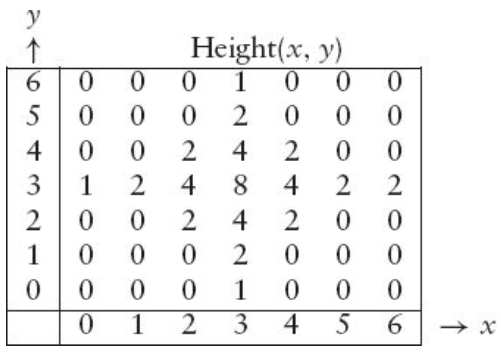
\includegraphics[width=3in]{img/PSet05hill.png}

\begin{parts}
\item Fit a not-a-knot cubic spline to the data in each row.  Then evaluate at the points $x = 0,0.1,0.2,...,5.9,6.0$ to create a $7\times 61$ array of values.

\emph{Use} \texttt{scipy.interpolate.CubicSpline} \emph{to create your spline fit.}
\item Fit a not-a-knot cubic spline to the data in each column of your $7\times 61$ array.  Evaluate these at $y = 0.0,0.1,0.2,...,5.9,6.0$ to produce a $61\times 61$ array of values.  Call this matrix $M$.
\item The code below has examples of two different ways to plot data from a 2D array.  Try each method for your data.
\begin{verbatim}
import numpy as np
from matplotlib import pyplot as plt
data = np.random.rand(61, 61)

# plot as an image
plt.imshow(data)
plt.show()

# surface plot
ax = plt.axes(projection='3d')
xvals = np.linspace(0,1,61)
x,y = np.meshgrid(xvals,xvals)
ax.plot_surface(x, y, data)
\end{verbatim}
\end{parts}


\item \emph{Time permitting} (Greenbaum and Chartier \S8.8 16)

PostScript and TrueType letters are created with splines using only a few points for each letter.  


The following code creates a letter from 7 data points.
\begin{verbatim}
import numpy as np
from scipy.interpolate import CubicSpline
import matplotlib.pyplot as plt

x = np.array([1, 2, 3, 2, 1.2, 2, 2.7])
y = np.array([1, 0, 1, 2.5, 3.4, 4, 3.2])
n = len(x)
t = np.arange(n)
delta = 0.01
tt = np.arange(0,n-1+delta,delta)
fx = CubicSpline(t,x)
fy = CubicSpline(t,y)

fig, ax = plt.subplots(1,1)
plt.plot(x,y,'o')
plt.plot(fx(tt),fy(tt))
ax.set_aspect('equal', 'box')    
\end{verbatim}

\begin{parts}
\item Create and print the letter defined by the following data.

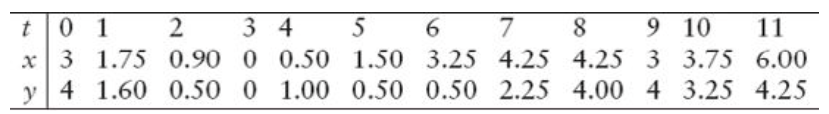
\includegraphics[width=0.6\textwidth]{img/PSet05letterdata.png}

\item On the same axes plot this letter along with the letter doubled in size.

\emph{\texttt{2*x} will double the size of the font in the $x$-direction.}

\item Create and print a different script letter.

\emph{Generate the $(t,x,y)$ values yourself - it's fine if your letter looks a little rough.}
\end{parts}






\item \emph{Time permitting} 

This is an extension topic: how to choose the spacing of the data points along the $x$-axis for polynomial interpolation to work as well as possible.


In the HumpherysJarvisBYU-ACME-LabsVolume2.pdf in the Additional Materials folder in the Files on Canvas, within the Polynomial Interpolation section, 

possibly Lab 9 problem 5

\end{questions}

\noindent\textbf{Extra information}

The structure of the final project:

 It will be based on a published paper.  You will work to understand and replicate key results.  Depending on the breadth and depth of the paper you will be expected to create a small extension or do a different exploration.
 
 I am providing a list of possible papers for this (\emph{see attached list}), or you can propose a paper.  There will be only one team per paper.

The default for the project will be to work in a team of three.  If there's a reason that a group of one, two, or four would work better, you'll have a chance to speak with me about arranging an exception. 

The teams will be assigned and the project proposals will be due later in October. %\textbf{Monday, April 1st}.  

A timeline for the project deliverables and more detailed expectations will be included in the next problem set.


\end{document}